\documentclass[]{article}
\usepackage{lmodern}
\usepackage{amssymb,amsmath}
\usepackage{ifxetex,ifluatex}
\usepackage{fixltx2e} % provides \textsubscript
\ifnum 0\ifxetex 1\fi\ifluatex 1\fi=0 % if pdftex
  \usepackage[T1]{fontenc}
  \usepackage[utf8]{inputenc}
\else % if luatex or xelatex
  \ifxetex
    \usepackage{mathspec}
  \else
    \usepackage{fontspec}
  \fi
  \defaultfontfeatures{Ligatures=TeX,Scale=MatchLowercase}
\fi
% use upquote if available, for straight quotes in verbatim environments
\IfFileExists{upquote.sty}{\usepackage{upquote}}{}
% use microtype if available
\IfFileExists{microtype.sty}{%
\usepackage[]{microtype}
\UseMicrotypeSet[protrusion]{basicmath} % disable protrusion for tt fonts
}{}
\PassOptionsToPackage{hyphens}{url} % url is loaded by hyperref
\usepackage[unicode=true]{hyperref}
\hypersetup{
            pdftitle={Revision},
            pdfborder={0 0 0},
            breaklinks=true}
\urlstyle{same}  % don't use monospace font for urls
\usepackage[margin=1in]{geometry}
\usepackage{graphicx,grffile}
\makeatletter
\def\maxwidth{\ifdim\Gin@nat@width>\linewidth\linewidth\else\Gin@nat@width\fi}
\def\maxheight{\ifdim\Gin@nat@height>\textheight\textheight\else\Gin@nat@height\fi}
\makeatother
% Scale images if necessary, so that they will not overflow the page
% margins by default, and it is still possible to overwrite the defaults
% using explicit options in \includegraphics[width, height, ...]{}
\setkeys{Gin}{width=\maxwidth,height=\maxheight,keepaspectratio}
\IfFileExists{parskip.sty}{%
\usepackage{parskip}
}{% else
\setlength{\parindent}{0pt}
\setlength{\parskip}{6pt plus 2pt minus 1pt}
}
\setlength{\emergencystretch}{3em}  % prevent overfull lines
\providecommand{\tightlist}{%
  \setlength{\itemsep}{0pt}\setlength{\parskip}{0pt}}
\setcounter{secnumdepth}{0}
% Redefines (sub)paragraphs to behave more like sections
\ifx\paragraph\undefined\else
\let\oldparagraph\paragraph
\renewcommand{\paragraph}[1]{\oldparagraph{#1}\mbox{}}
\fi
\ifx\subparagraph\undefined\else
\let\oldsubparagraph\subparagraph
\renewcommand{\subparagraph}[1]{\oldsubparagraph{#1}\mbox{}}
\fi

% set default figure placement to htbp
\makeatletter
\def\fps@figure{htbp}
\makeatother

\usepackage{xcolor}

\title{Revision}
\author{}
\date{\vspace{-2.5em}}

\begin{document}
\maketitle

\subsection{Reviewer 1}\label{reviewer-1}

\subsubsection{Question about number of clusters at each
condition}\label{question-about-number-of-clusters-at-each-condition}

\begin{enumerate}
\def\labelenumi{(\arabic{enumi})}
\tightlist
\item
  One key assumption they made is that the number of cell clusters in
  both conditions is the same (K). This does not allow the scenarios
  where different conditions may have different cell subtypes (e.g.,
  normal versus controls). Of course, if the cell types are different,
  then all genes should have different distributions. Should not they
  first decide whether this is the case?
\end{enumerate}

\textcolor{blue}{It is not an assumption for number of clusters to be same across two conditions. Our method pooled cells from both conditions first and identified a global clustering for all the cells, the number of clusters ($K$) is for the global clustering. These two conditions can have different number of clusters given that one condition can have zero proportion of cells from a cluster.
For example, $K = 3$, there are 3 clusters (labelled as A, B, C) globally. Condition 1 having 3 types, 60\% from A, 30\% from B and 10\% from C, while condition 2 only have 2 types 50\% from B and 50\% from C.}
\textcolor{blue}{It is not necessary that different cell types will induce different distributions over the whole genome. Actually the major proportion of genes should still have equivalent distribution. 
Which is key observation we proposed in the paper and we propose an empirical Bayesian framework with a specifically constructed prior to handle the scenario when both means and proportions changed.}

\subsubsection{Questions about fitting data with mixture of
NB}\label{questions-about-fitting-data-with-mixture-of-nb}

\begin{enumerate}
\def\labelenumi{(\arabic{enumi})}
\setcounter{enumi}{1}
\tightlist
\item
  Single cell RNA-seq data often have lots of zeros. I was wondering how
  well the mixture of multinomial distributions really fit the data.
  Some plots that show the model fits would be useful.
\end{enumerate}

\textcolor{blue}{We are using mixture of negative binomial to model the counts instead of multinomial distributions. Mixture of NB are flexible to approximate a lot of distributions. Specifically, NB can approximate constant 0 by arbitrary accuracy. As we know the density of $P(X = 0) = 1 - p$ and $P(X > 0) = p$ given $X \sim \text{NB}(1,p)$. Further, scRNA-seq data tends to be overdispersed so that many people are using NB to model it. (cite DESeq2, cite Normalization and variance stabilization of single-cell RNA-seq data using regularized negative binomial regression). Also, the empirical data (EMTAB2805, GSE45719) showed that more than 80\% of genes their nonzero counts are overdispersed. In addition, given our estimated group labels, we test whether there is a strong evidence to reject fitting NB model at each group. Given the cells from same group, we excluded those genes with more than 70\% of 0s, as we know NB can approximate 0 well. For the remaining genes, we do the goodness of fit tests following the procedure proposed in the paper "Pearson-type goodness-of-fit test with
bootstrap maximum likelihood
estimation(Guosheng Yin,Yanyuan Ma)". We found very few genes would reject the negative binomial model
} 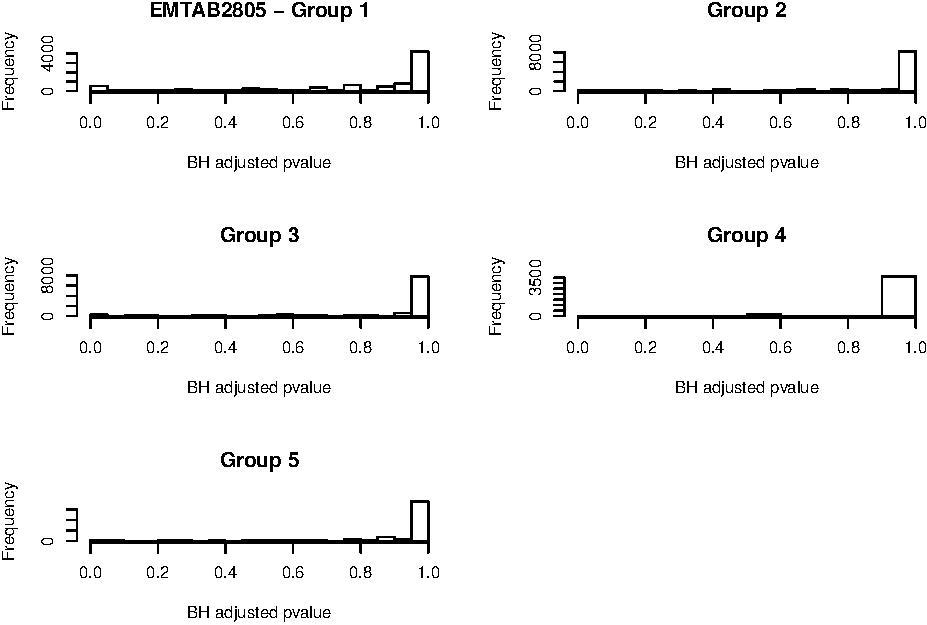
\includegraphics{Revision_files/figure-latex/unnamed-chunk-1-1.pdf}
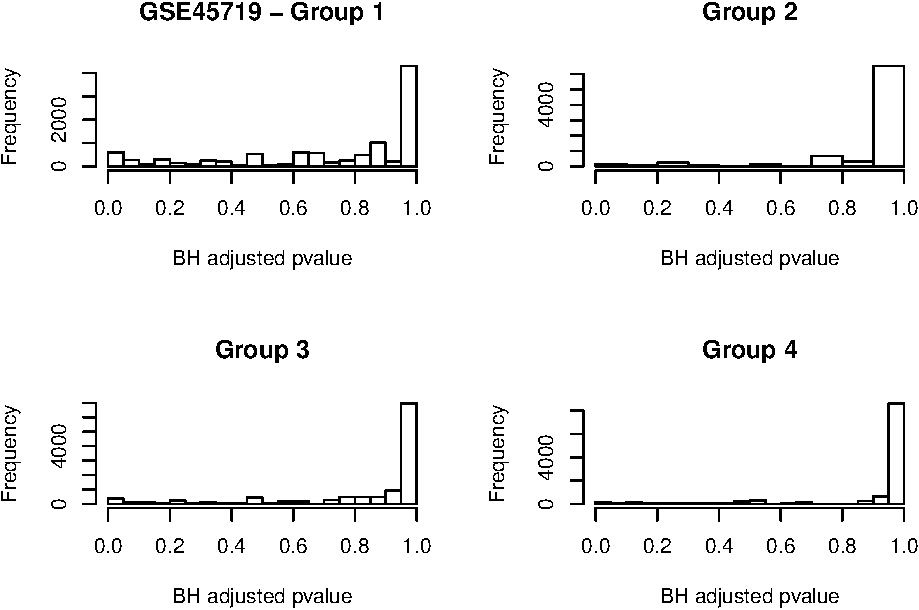
\includegraphics{Revision_files/figure-latex/unnamed-chunk-1-2.pdf}

\subsubsection{Questions not sure}\label{questions-not-sure}

(3). For the transcriptional bursting data analysis,\\
some comparisons with other methods such as MAST, DESEQ2, scDD would be
useful, as they did for synthetic data sets.

\subsection{Reviewer 2}\label{reviewer-2}

\subsubsection{Questions not sure}\label{questions-not-sure-1}

1.How does the model behave when both the proportions and the means are
different? The calculation p7 (before the key issue) should be detailed.
What hypotheses on \(f_{g,k}\) allow this result ? The distribution can
remain the same even both proportions and means changed. We assume the
only parameter differs \(f_{g,k}\) for \(k\) is the mean.

\textcolor{blue}{The distribution can remain the same even both proportions and means changed. 
We assume the only parameter differs $f_{g,k}$ for $k$ is the mean.}

2.It is assumed that the shape parameter is constant and independent to
the population classes. Is it a realistic hypothesis ? What is it impact
on the results ? Is it possible to relax this hypothesis to consider a
shape parameter depending on \(k\) ? A discussion on this hypothesis
should be added in the discussion.

\textcolor{blue}{For the fixed shape parameter of NB among groups, we performed tests on each gene.
The testing procedure is following: the null hypothesis is for different groups having the same shape parameter. Under the null we pool the data and find the MLE and obtain it's condifence interval by fisher information. Under alternative, we use MLE to obtain point estimator of shape parameter separately at each group. If there is at least one group's point estimator being outside of the confidence interval, we flagged the corresponding gene. We run the test on the GSE75748. We found 1185 out of 19097 genes (6.2\%) having been identified as genes with hetergenous shape parameters. 
So for the majority of genes, it is ok to assume a shared shape parameter across groups.
Further, our aim is to infer the distribution pattern of mixing components. If for some genes and some groups both mean and shape parameters are different. It may still be ok only testing the change pattern of means. Among those 1185 flagged genes, 690 of them also shows differential means for its max posterior given by EBSeq, which further reduce the effects of unequal shape parameter.
We also run the same procedure on GSE45719. We found 3\% genes having been flagged and 73\% among them are also having differential means between groups. I would say overall the proportion of genes may be affected by the same shape parameter assumption is low 
}

\subsubsection{Question about sensitivity to
clustering}\label{question-about-sensitivity-to-clustering}

3.For the clustering, the authors should better justify their choice.
The results seem to be strongly related to the clustering method.

\textcolor{blue}{We have tried different clustering method, sc3 on 3 datasets, (EBTAB2805, GSE45719, GSE79102). 
the correlation coefficients of the local fdr are 0.92,0.94,0.96. Our method is not very sensitive to the clustering methods.}

\subsubsection{Questions for
simulations}\label{questions-for-simulations}

Finally for the simulation part, the data generation should be explained
and it would be nice to have criteria evaluating the difficulty of the
simulated datasets. For example \(K=12\) seems very difficult, and
\(K=7\) also (On Figure S7, some ROC curves are closed to the first
bisector. Moreover on this plot, configurations are not precised).

\textcolor{blue}{More detailed information of simulation has been placed in the supplementary material, those pca plots showed that groups are collapsed together when there are more groups, which make all the methods difficult to detect DD genes. In addition, we have fixed number of cells(400) so more number of groups will decrease the number of cells per group which makes it harder to detect the change between groups also mixing of more groups weaken the overall signal between conditions.
Further to show the difficulty of each simulation settings, we do a t-test on each gene and present a boxplot for every simulation settings. It is easier to detect DD genes if they having small p values compare to those of ED genes, we ordered the boxplot by the same order of the simulation graph in the paper (Fig 4)}

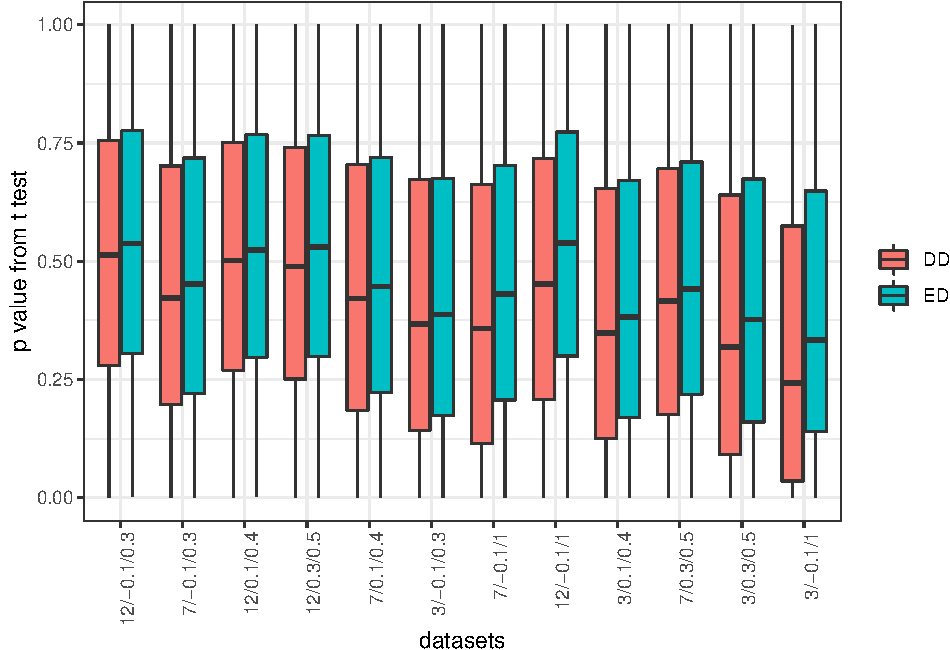
\includegraphics{Revision_files/figure-latex/unnamed-chunk-2-1.pdf}

\subsubsection{Questions for
simulations}\label{questions-for-simulations-1}

The results on Figures 4 and 5 are questionable. ScDDboost has the best
TPR and a FDR closed to 0, whereas this latter should be controled at
5\%. DESeq2 seems to better control the trade-off. Can the authors
comment this remark ? In general, I am very surprised by the very small
number of replicate datasets per scenario. Is it possible to increase it
and to use boxplots and ROC curves to summary the results instead of one
figure for the TPR and one figure for the FDR ?

\textcolor{blue}{We have done more replicates for each simulation setting, now we have 10 replicates under each settings. And we have similar results as before. (add plots later)\\
Our method is not a trade-off for more power by using FDR.}

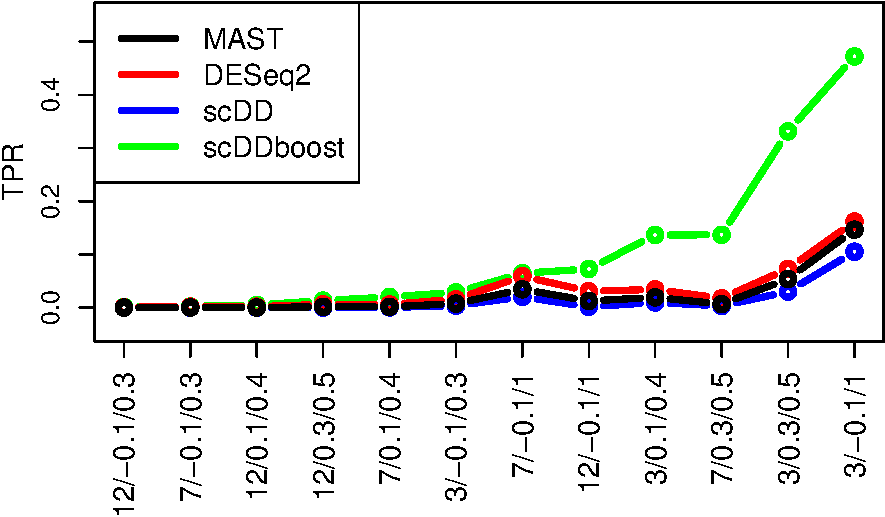
\includegraphics{Revision_files/figure-latex/unnamed-chunk-3-1.pdf}

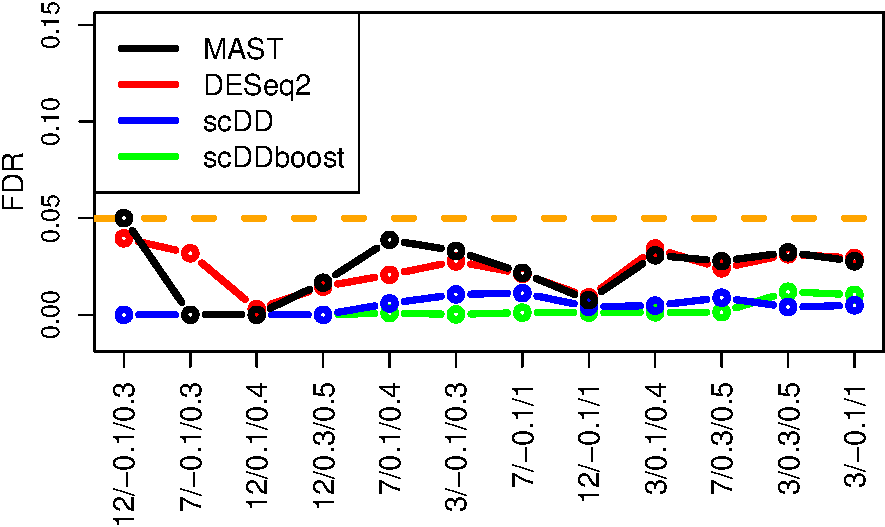
\includegraphics{Revision_files/figure-latex/unnamed-chunk-4-1.pdf}

\end{document}
